% !TeX program = xelatex
% Exactly 12 frames. Source notes are hidden in the presentation PDF.
\documentclass[aspectratio=169,10pt]{beamer}
\usepackage[UTF8,fontset=fandol]{ctex}
\usepackage{fontspec,graphicx,tikz,booktabs,array}
\setsansfont{texgyreheros-regular.otf}[BoldFont=texgyreheros-bold.otf,ItalicFont=texgyreheros-italic.otf]
\IfFontExistsTF{PingFang SC}{%
  \setCJKsansfont{PingFang SC}[BoldFont={PingFang SC Semibold}]%
}{\IfFontExistsTF{Noto Sans CJK SC}{%
  \setCJKsansfont{Noto Sans CJK SC}[BoldFont={Noto Sans CJK SC Bold}]%
}{\setCJKsansfont{FandolHei-Regular.otf}[BoldFont=FandolHei-Bold.otf]}}
\setmonofont{texgyrecursor-regular.otf}
\definecolor{Ink}{HTML}{153A57}
\definecolor{Muted}{HTML}{647583}
\definecolor{Teal}{HTML}{087F8C}
\definecolor{Orange}{HTML}{D48538}
\definecolor{Hairline}{HTML}{DCE5EB}
\definecolor{Paper}{HTML}{F5F7F9}
\xeCJKsetup{CJKglue={\hskip 0pt},CJKecglue={\hskip 0.13em}}
\setbeamercolor{normal text}{fg=Ink,bg=white}
\setbeamercolor{background canvas}{bg=white}
\setbeamertemplate{navigation symbols}{}
\setbeamertemplate{footline}{}
\setbeameroption{hide notes}
\hypersetup{pdftitle={KSSOLV Toolbox V0.5.0},pdfauthor={KSSOLV Toolbox},pdfsubject={12页中文Beamer演示稿}}
% TikZ positions text and supplied screenshots. Sources remain in hidden notes.
\newenvironment{canvas}{\begin{tikzpicture}[remember picture,overlay]\begin{scope}[shift={(current page.north west)},x=1cm,y=-1cm]}{\node[anchor=south east,inner sep=0,text=Muted,font=\fontsize{8}{10}\selectfont] at (15.2,8.77) {\insertframenumber};\end{scope}\end{tikzpicture}}
\newcommand{\txt}[4]{\node[anchor=north west,inner sep=0,text width=#3cm,align=left] at (#1,#2) {#4};}
\newcommand{\ctxt}[4]{\node[anchor=north,inner sep=0] at (#1,#2) {\mbox{#4}};}
\newcommand{\shot}[5]{\node[anchor=center,inner sep=0] at ({#1+#3/2},{#2+#4/2}) {\includegraphics[width=#3cm,height=#4cm,keepaspectratio]{images/#5}};}
\newcommand{\head}[1]{\txt{0.8}{0.55}{14.4}{\fontsize{18}{23}\selectfont\bfseries #1}\draw[Hairline,line width=0.35pt] (0.8,1.42)--(15.2,1.42);}
\newcommand{\bodyfont}{\fontsize{11.5}{16}\selectfont}
\newcommand{\captionfont}{\fontsize{11.3}{15}\selectfont\bfseries}
\newcommand{\catalogue}[5]{\txt{#1}{#2}{#3}{\fontsize{10.2}{13}\selectfont\bfseries\color{Teal}#4}\txt{#1}{#2+0.45}{#3}{\fontsize{8.9}{11.6}\selectfont #5}}
\newcommand{\topic}[5]{\txt{#1}{#2}{#3}{\fontsize{11.5}{15}\selectfont\bfseries\color{Teal}#4\par\vspace{0.18cm}\color{Ink}\normalfont\fontsize{10.3}{14.5}\selectfont #5}}
\newcommand{\cell}[4]{\txt{#1}{#2}{#3}{\fontsize{10.1}{14.2}\selectfont #4}}
\begin{document}

\begin{frame}[plain]
\begin{canvas}
\shot{7.8}{1.10}{7.65}{6.8}{cover-molecule.jpg}
\txt{0.9}{1.55}{6.7}{\fontsize{36}{40}\selectfont\bfseries KSSOLV}
\txt{0.9}{2.95}{6.7}{\fontsize{30}{35}\selectfont Toolbox}
\txt{0.94}{4.38}{6.2}{\color{Teal}\fontsize{18}{23}\selectfont V0.5.0}
\txt{0.94}{5.88}{6.3}{\fontsize{15}{23}\selectfont 材料建模与\par 第一性原理计算}
\end{canvas}
\note{v.04.0对应V0.4.0。当前版本按KSSOLV\_Toolbox.m的Version=0.5.0确定。最新本地标签为V0.4.1，HEAD=40369fd，工作区含未提交内容。不能把当前工作区等同于已打标签发布版。图为实际查看器中的吡啶初始模型。}
\end{frame}

\begin{frame}[plain]
\begin{canvas}
\head{分子与晶体的交互建模}
\filldraw[fill=white,draw=Hairline,line width=0.35pt] (0.8,1.9) rectangle (7.7,7.05);
\filldraw[fill=white,draw=Hairline,line width=0.35pt] (8.3,1.9) rectangle (15.2,7.05);
\shot{0.84}{1.94}{6.82}{5.07}{modeling-ui.jpg}
\node[anchor=center,inner sep=0] at (11.75,4.475) {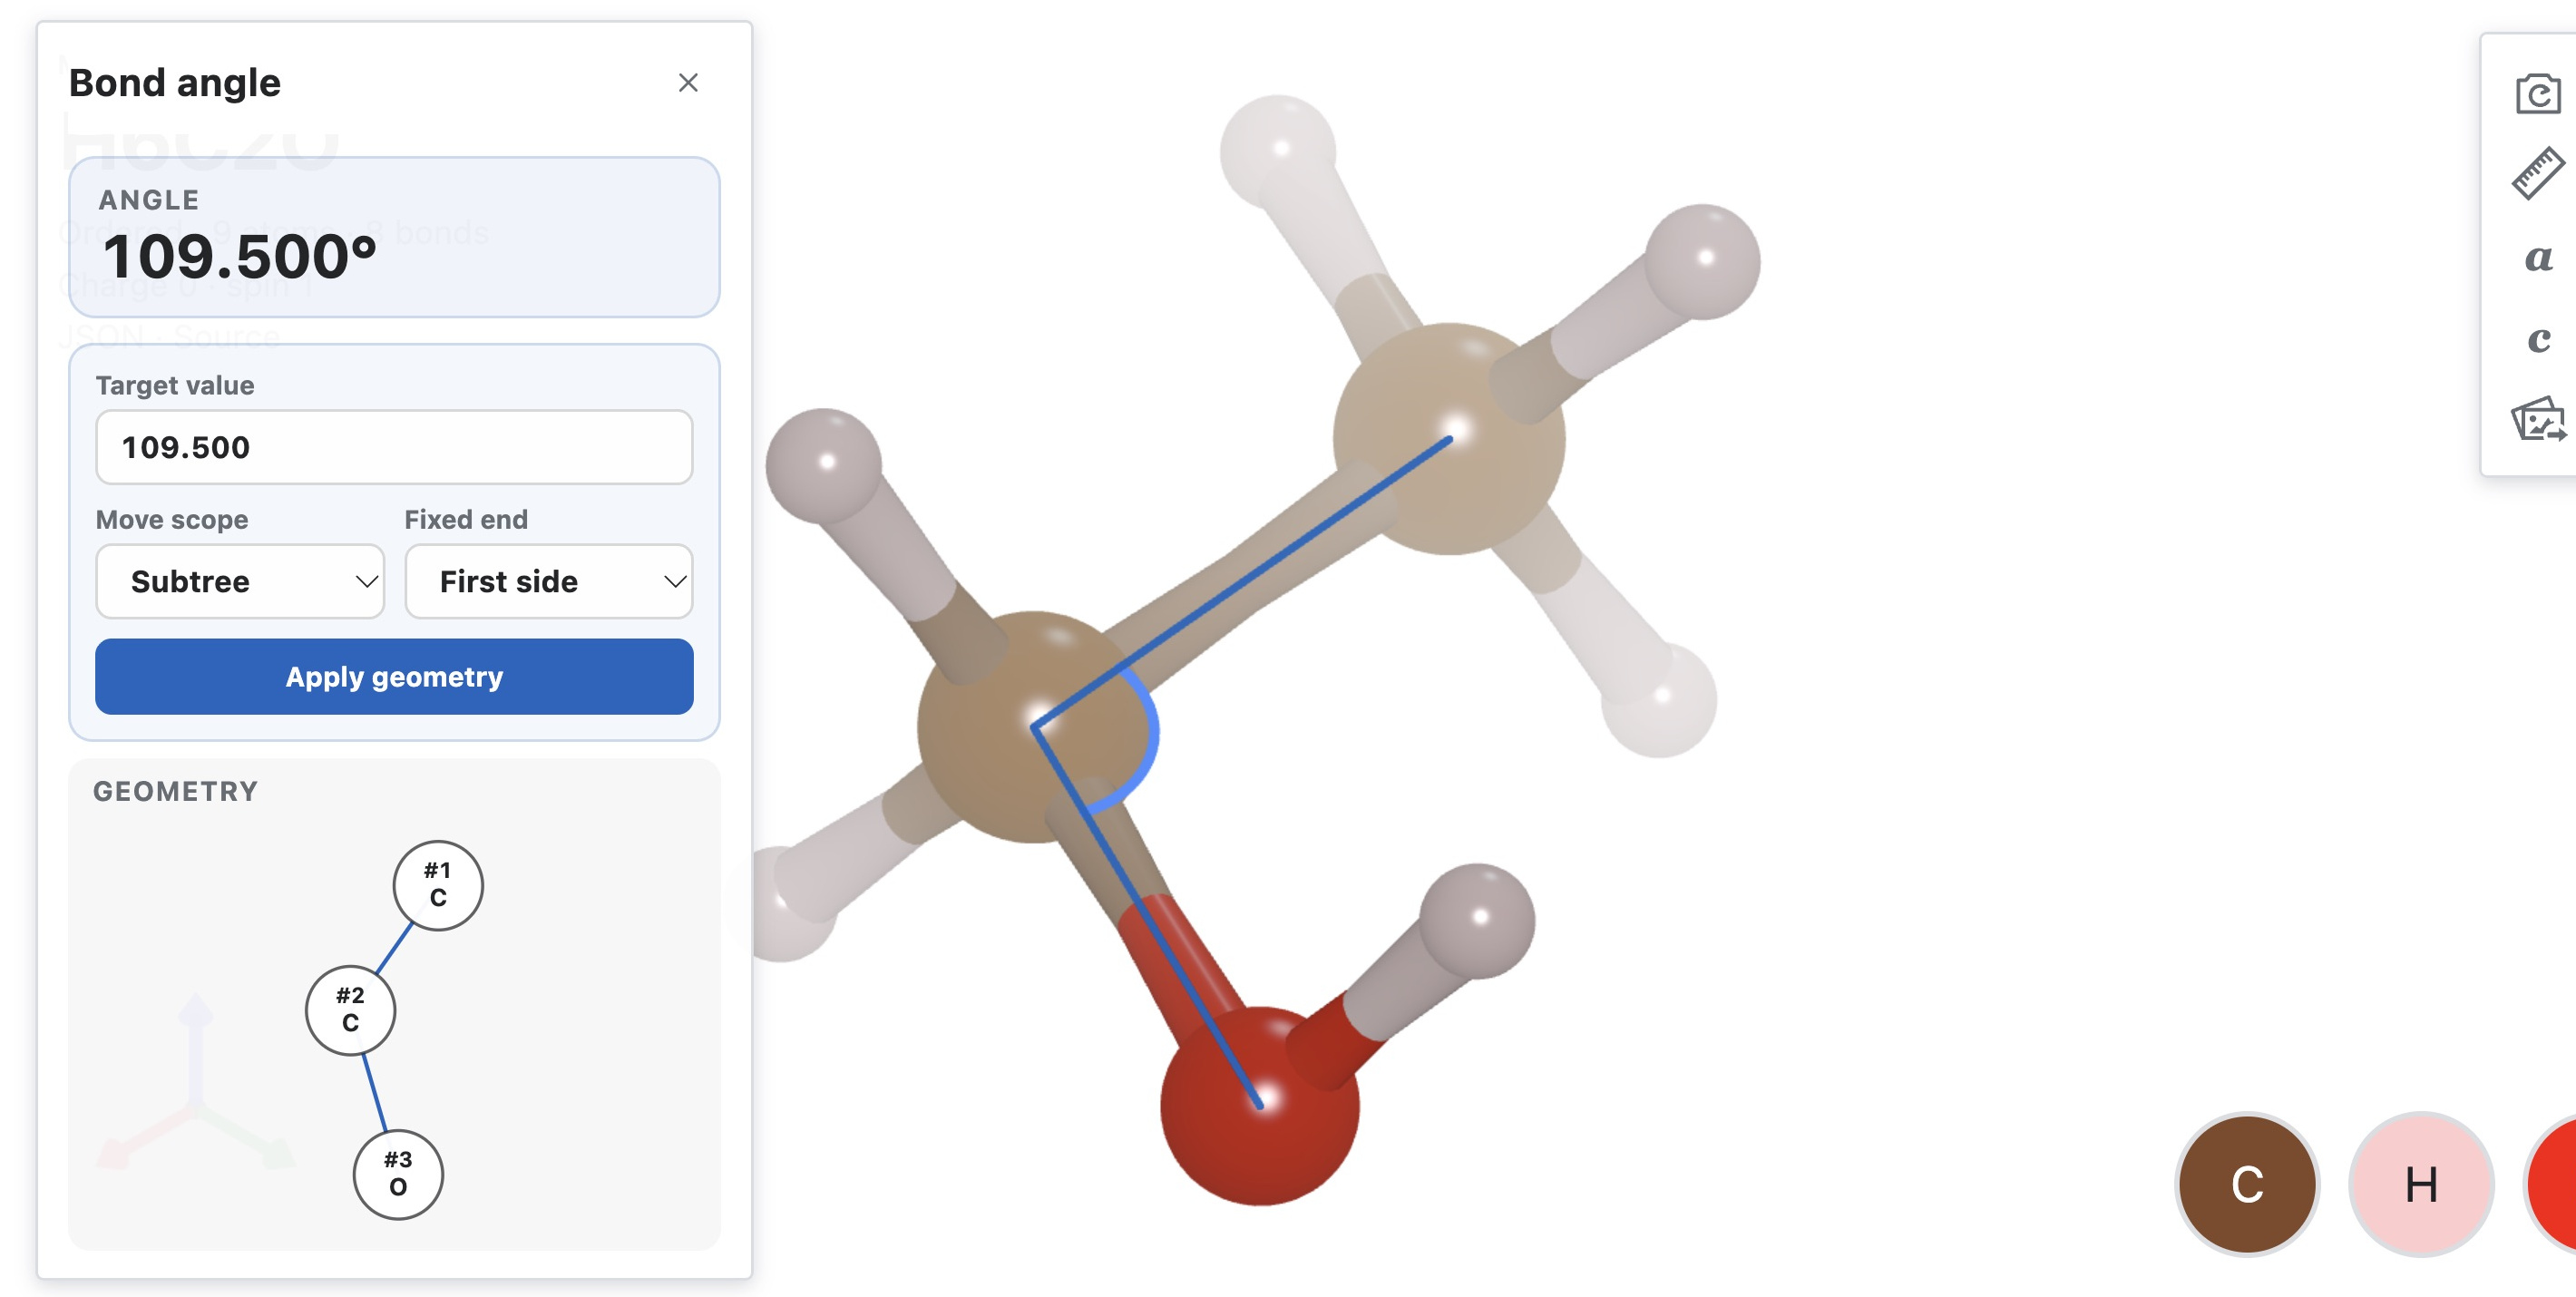
\includegraphics[trim=0 0 650 0,clip,width=6.72cm,height=4.95cm,keepaspectratio]{images/angle-edit.jpg}};
\txt{0.8}{7.48}{6.9}{\captionfont 晶体结构编辑}
\txt{8.3}{7.48}{6.9}{\captionfont 分子几何编辑}
\end{canvas}
\note{来源docs/modeling-user-guide.zh-CN.md、ModelingTab.m。支持选择、移动旋转、3D草绘、显式拓扑、补氢、几何编辑、预览和撤销。左为Al2O3工作区，右为乙醇角度编辑；109.500度为编辑目标，不是优化平衡角。}
\end{frame}


\begin{frame}[plain]
\begin{canvas}
\head{建模功能全览}
\txt{10.15}{0.69}{5.05}{\fontsize{11.2}{15}\selectfont\color{Teal}10 类 / 75 项命令}
\catalogue{0.8}{1.72}{6.85}{原子编辑\quad 12 项}{添加、删除、替换、合并、固定、居中\\排序、移动、平移、旋转、镜像、扰动}
\catalogue{0.8}{3.05}{6.85}{分子建模\quad 18 项}{原子与环草绘，化学键增删与键级\\化学属性、补氢去氢、诊断与测量\\键长、键角、二面角，对齐与几何整理\\几何优化、片段连接、用户片段保存}
\catalogue{0.8}{5.20}{6.85}{晶格编辑\quad 5 项}{参数编辑、应变、镜像、旋转与轴交换}
\catalogue{0.8}{6.13}{6.85}{超胞与晶格\quad 5 项}{超胞、重定义、正交化、结构应变与扰动}
\catalogue{0.8}{7.06}{6.85}{对称性工具\quad 6 项}{空间群构建、P1、对称性分析\\原胞、惯用胞、Wigner-Seitz 晶胞}
\catalogue{8.35}{1.72}{6.85}{聚合物建模\quad 6 项}{均聚、嵌段、无规、支化、基础树枝状\\自定义重复单元保存}
\catalogue{8.35}{3.05}{6.85}{无定形建模\quad 5 项}{非晶晶胞、混合物装填、受限分子层\\已有晶胞装填、纳米颗粒周围装填}
\catalogue{8.35}{4.40}{6.85}{缺陷与合金\quad 3 项}{点缺陷创建、不等价缺陷枚举、SQS}
\catalogue{8.35}{5.34}{6.85}{纳米结构\quad 4 项}{纳米管、纳米带、纳米线、量子点与空洞}
\catalogue{8.35}{6.28}{6.85}{表面与界面\quad 11 项}{表面、真空层、结构插入、异质堆叠\\扭转莫尔结构、NEB 插值、吸附位点\\吸附构型搜索与放置、钝化、溶剂层}
\end{canvas}
\note{按当前+kssolv/+modeling/CommandCatalog.m的10类75项公开命令完整分组；中文名称核对zh\_CN/modeling.xml。不是对所有75项逐一运行验收。modeling-inventory.json保存每个command ID、中文标签及分类计数。分子几何优化使用kssolv-generic-mm-v2，基础树枝状聚合物按实际命令标签标注。}
\end{frame}


\begin{frame}[plain]
\begin{canvas}
\head{复杂材料结构构建}
\shot{0.8}{1.83}{4.45}{3.95}{defect-model.jpg}
\shot{5.775}{1.83}{4.45}{3.95}{surface-oh.jpg}
\shot{10.75}{1.83}{4.45}{3.95}{twist-model.jpg}
\ctxt{3.025}{5.99}{4.45}{\captionfont 缺陷超胞}
\ctxt{8}{5.99}{4.45}{\captionfont 表面吸附}
\ctxt{12.975}{5.99}{4.45}{\captionfont 扭转双层结构}
\shot{1.1}{6.60}{13.8}{1.38}{polymer-chain.jpg}
\ctxt{8}{8.17}{13.8}{\captionfont 高分子链构建}
\end{canvas}
\note{来源建模指南及+modeling各builder。图为硅空位、Pt表面OH初始放置、扭转石墨烯和高分子初始链。吸附几何评分不是吸附能，需进一步弛豫。聚合物和装填结构需最小化/平衡。不把周期映像显示数量当独立位点数。}
\end{frame}


\begin{frame}[plain]
\begin{canvas}
\head{与 Materials Studio 的功能对照}
\cell{0.92}{1.86}{2.0}{\bfseries 比较维度}
\cell{3.25}{1.86}{5.4}{\bfseries\color{Teal}KSSOLV Toolbox}
\cell{9.3}{1.86}{5.75}{\bfseries Materials Studio}
\draw[Hairline,line width=.5pt] (0.8,2.46)--(15.2,2.46);
\fill[Paper] (0.8,2.48) rectangle (15.2,3.42);
\fill[Paper] (0.8,4.42) rectangle (15.2,5.36);
\fill[Paper] (0.8,6.36) rectangle (15.2,7.30);
\cell{0.92}{2.65}{2.0}{结构构建}
\cell{3.25}{2.65}{5.4}{分子、晶体、表面、高分子}
\cell{9.3}{2.65}{5.75}{Visualizer\\分子、晶体、表面、聚合物}
\cell{0.92}{3.62}{2.0}{复杂体系}
\cell{3.25}{3.62}{5.4}{缺陷、SQS、扭转结构、非晶装填}
\cell{9.3}{3.62}{5.75}{纳米结构与层构建\\Amorphous Cell 装填}
\cell{0.92}{4.60}{2.0}{几何与力场}
\cell{3.25}{4.60}{5.4}{通用分子模型\\初始几何准备}
\cell{9.3}{4.60}{5.75}{Forcite Plus\\力场优化与分子动力学}
\cell{0.92}{5.59}{2.0}{电子结构}
\cell{3.25}{5.59}{5.4}{KSSOLV 平面波 DFT 工作流}
\cell{9.3}{5.59}{5.75}{CASTEP、DMol$^3$ 等 DFT 模块}
\cell{0.92}{6.57}{2.0}{自动化接口}
\cell{3.25}{6.57}{5.4}{MATLAB API 与计算工作流}
\cell{9.3}{6.57}{5.75}{MaterialsScript 与 Pipeline Pilot}
\cell{0.92}{7.55}{2.0}{部署形态}
\cell{3.25}{7.35}{5.4}{桌面应用、远程集群\\\mbox{KSSOLV Toolbox Online}}
\cell{9.3}{7.55}{5.75}{桌面客户端/服务器与云平台}
\draw[Hairline,line width=.5pt] (0.8,8.36)--(15.2,8.36);
\end{canvas}
\note{对照为功能范围与方法定位，不表示算法、精度、力场完备性或性能相同。KSSOLV侧依据README、CommandCatalog和MolecularMechanicsForceField.m；通用分子模型不含静电和色散吸引。Materials Studio侧依据Dassault Systemes官方Visualizer数据表\url{https://www.3ds.com/fileadmin/PRODUCTS-SERVICES/BIOVIA/PDF/materials-studio-visualizer.pdf}与官方产品总览\url{https://www.3ds.com/assets/invest/2023-10/biovia-materials-studio-overview.pdf}，2026-10-22查阅。Forcite Plus、Amorphous Cell、CASTEP、DMol3是不同模块；未假定某一种许可包含全部模块。未对Materials Studio运行基准。云平台产品以官方产品主页为证据：\url{https://www.3ds.com/products/biovia/materials-studio}。}
\end{frame}


\begin{frame}[plain]
\begin{canvas}
\head{三维体数据可视化}
\shot{0.35}{1.90}{5.3}{5.15}{volume-iso.jpg}
\shot{5.35}{1.90}{5.3}{5.15}{volume-miller.jpg}
\shot{10.35}{1.90}{5.3}{5.15}{volume-dvr.jpg}
\ctxt{3}{7.38}{4.8}{\captionfont 等值面}
\ctxt{8}{7.38}{4.8}{\captionfont 晶面切片}
\ctxt{13}{7.38}{4.8}{\captionfont 直接体渲染}
\end{canvas}
\note{来源docs/volume-viewer-user-guide.zh-CN.md。真实体数据截图演示不同观察模式，不作同通道同阈值定量比较。支持自旋通道、非正交网格、原子叠加、PNG和几何导出。WebGL2或三维纹理不可用可降级CPU切片，GPU体渲染不等于DFT计算在GPU执行。}
\end{frame}

\begin{frame}[plain]
\begin{canvas}
\head{计算工作流与执行资源}
\shot{0.8}{1.84}{6.05}{4.95}{workflow-graph.jpg}
\shot{7.45}{1.84}{7.75}{4.95}{scf-result.jpg}
\ctxt{3.825}{7.00}{6.05}{\captionfont SCF、能带与态密度}
\ctxt{11.325}{7.00}{7.75}{\captionfont SCF 收敛与结果分析}
\draw[Hairline,line width=.35pt] (0.8,7.85)--(15.2,7.85);
\ctxt{8}{8.13}{14.4}{\fontsize{11}{15}\selectfont\color{Teal}串行计算\qquad 进程并行\qquad GPU 计算}
\end{canvas}
\note{左为能带工作流，右为真实独立应用H2 SCF曲线，二者不是同一体系。当前README-zh.md与ExecutionResources.m说明支持串行、受限进程池和指定算法GPU。SCF/NSCF/能带/DOS的lobpcg、davidson、davidson2、davpcg提供GPU路径，NSCF/能带/DOS可配置进程池，能带和DOS可继承NSCF设置。HT插值不走这些并行路径，三维能带直接调用NSCF。没有实测加速倍数。}
\end{frame}

\begin{frame}[plain]
\begin{canvas}
\head{远程计算的四种执行模式}
\txt{0.95}{2.0}{3.0}{\color{Teal}\fontsize{54}{59}\selectfont\bfseries 4}
\txt{1.03}{4.22}{3.3}{\fontsize{15}{21}\selectfont 执行模式}
\txt{1.03}{5.52}{3.3}{\bodyfont 作业提交}
\txt{1.03}{6.20}{3.3}{\bodyfont 状态跟踪}
\txt{1.03}{6.88}{3.3}{\bodyfont 结果回传}
\txt{5.00}{2.02}{2.5}{\fontsize{13}{18}\selectfont\bfseries Standard}
\txt{7.80}{2.02}{7.1}{\bodyfont 本地 MATLAB 提交至集群}
\txt{5.00}{3.48}{2.5}{\fontsize{13}{18}\selectfont\bfseries Bridge}
\txt{7.80}{3.48}{7.1}{\bodyfont 远端 MATLAB 代理提交}
\txt{5.00}{4.94}{2.5}{\fontsize{13}{18}\selectfont\bfseries Mirror}
\txt{7.80}{4.94}{7.1}{\bodyfont 远端 MATLAB 单进程执行}
\txt{5.00}{6.40}{2.5}{\fontsize{13}{18}\selectfont\bfseries Cloud}
\txt{7.80}{6.40}{7.1}{\bodyfont 使用 MATLAB Cluster Profile}
\foreach \y in {2.93,4.39,5.85,7.31}{\draw[Hairline,line width=.35pt] (5.0,\y)--(15.2,\y);}
\end{canvas}
\note{来源docs/remote-computing-user-guide.zh-CN.md及V0.4.0远程服务README。Standard要求本地MATLAB、Parallel Server、worker同release；Bridge要求远端MATLAB及worker同release；Mirror不要求Parallel Server，仍需MATLAB许可；Cloud使用已有可用Profile。本地均需Parallel Computing Toolbox。页面是模式映射表，不表示本次连接或验证了任何集群。}
\end{frame}

\begin{frame}[plain]
\begin{canvas}
\head{独立应用与运行环境}
\shot{0.8}{1.83}{10.25}{6.33}{startup-card.jpg}
\topic{11.65}{2.24}{3.55}{独立安装包}{Windows / macOS}
\topic{11.65}{4.16}{3.55}{运行环境}{MATLAB Runtime}
\topic{11.65}{6.08}{3.55}{首次启动}{安装后预热}
\end{canvas}
\note{来源scripts/windows/README.zh-CN.md、scripts/startup/README.md、buildInstaller.m及安装提交。Windows使用Inno Setup和Runtime预热，macOS提供PKG与Runtime分发。本页为实际V0.5.0启动卡片，省略旧版本安装器截图。插画为既有产品美术资产，不是DFT数据。构建文档使用-nojvm，本次未重新运行Toolbox或作Java约束验收。}
\end{frame}


\begin{frame}[plain]
\begin{canvas}
\head{文档与示例}
\filldraw[fill=Paper,draw=Hairline,line width=.35pt] (0.8,1.77) rectangle (5.4,8.22);
\shot{1.01}{1.99}{4.18}{6.0}{documentation-cover.png}
\topic{6.2}{1.95}{4.25}{中英文使用指南}{安装与结构建模\\工作流与结果分析}
\topic{10.95}{1.95}{4.25}{配套实例与复算材料}{分子、晶体与表面\\能带与体数据示例}
\topic{6.2}{4.18}{4.25}{建模与接口参考}{75 项建模命令\\Modeling API 与结构 I/O}
\topic{10.95}{4.18}{4.25}{部署与运维说明}{独立应用与远程计算\\\mbox{KSSOLV Toolbox Online}\\管理与部署}
\draw[Hairline,line width=.35pt] (6.2,7.00)--(15.2,7.00);
\txt{6.2}{7.25}{9.0}{\fontsize{10.1}{14}\selectfont\color{Teal}\href{https://github.com/USTC-Hu-Group/KSSOLV-Toolbox}{\underline{代码仓库\quad USTC-Hu-Group/KSSOLV-Toolbox}}}
\txt{6.2}{7.93}{9.0}{\fontsize{10.1}{14}\selectfont\color{Teal}\href{https://github.com/USTC-Hu-Group/KSSOLV-Toolbox-Manual}{\underline{用户文档\quad USTC-Hu-Group/KSSOLV-Toolbox-Manual}}}
\end{canvas}
\note{来源docs/README.md、docs/manual-zh/main.tex、chapters/00-frontmatter.tex、examples目录，以及scripts/docker和scripts/k8s文档。中文手册封面从现有manual-style.sty的manualcover重新渲染，内容未改写，仅使用可正常嵌入的本机中文字体；未修改既有手册源文件。中英文指南指仓库中确有的Markdown使用指南，封面为中文用户手册，不声称存在已验收的英文完整PDF。仓库链接为\url{https://github.com/USTC-Hu-Group/KSSOLV-Toolbox}，文档入口为\url{https://github.com/USTC-Hu-Group/KSSOLV-Toolbox-Manual}，2026-10-22核对仓库origin；用户文档采用用户指定并核实的独立手册仓库。}
\end{frame}



\begin{frame}[plain]
\begin{canvas}
\head{\mbox{KSSOLV Toolbox Online}：建模与计算}
\shot{0.8}{1.87}{9.50}{5.45}{online-files.jpg}
\topic{10.95}{2.02}{4.25}{独立工作空间}{按用户隔离\\已保存文件持久存储}
\topic{10.95}{3.96}{4.25}{建模与计算}{结构编辑与 SCF\\在线查看计算结果}
\topic{10.95}{5.90}{4.25}{会话恢复}{工作空间重连\\重启后读取已存文件}
\draw[Hairline,line width=.35pt] (0.8,7.78)--(15.2,7.78);
\ctxt{3.0}{8.12}{4.4}{\fontsize{11}{15}\selectfont 小\quad 2 核 / 8 GiB}
\ctxt{8.0}{8.12}{4.4}{\fontsize{11}{15}\selectfont 中\quad 4 核 / 24 GiB}
\ctxt{13.0}{8.12}{4.4}{\fontsize{11}{15}\selectfont 大\quad 8 核 / 52 GiB}
\end{canvas}
\note{来源scripts/k8s/README.zh-CN.md与scripts/docker/README.zh-CN.md。所列小中大为文档默认档位，可由管理员调整，不代表实时可用额度。每用户独立namespace、Runtime和PVC，每个Runtime仅支持一个活动浏览器客户端。持久保存指已保存文件和设置；临时界面状态与未保存计算内容不保证恢复。Runtime内部接口需随MATLAB发行版回归，GPU和完整跨平台仍有验证边界。本次使用已有实际工作区截图，不启动、扩缩容或重启工作空间。}
\end{frame}



\begin{frame}[plain]
\begin{canvas}
\head{\mbox{KSSOLV Toolbox Online}：资源与运维}
\filldraw[fill=white,draw=Hairline,line width=.35pt] (0.8,1.85) rectangle (9.95,4.74);
\filldraw[fill=white,draw=Hairline,line width=.35pt] (0.8,5.16) rectangle (9.95,8.23);
\shot{0.84}{1.89}{9.07}{2.81}{online-admin-users-crop.png}
\shot{0.84}{5.20}{9.07}{2.99}{online-admin-cpu.png}
\topic{10.65}{1.99}{4.55}{用户与权限}{账号角色、冻结与恢复}
\topic{10.65}{3.62}{4.55}{实例与资源}{资源档位、实例生命周期}
\topic{10.65}{5.25}{4.55}{监控与核时}{资源曲线、核时与审计}
\topic{10.65}{6.88}{4.55}{运维自动化}{节点维护、脚本定期执行}
\end{canvas}
\note{来源scripts/k8s/admin/README.zh-CN.md及2026-10-22已打开的真实管理页。截图只读采集用户核时表和已有实例CPU曲线；没有修改账号、权限、资源配置、邀请码或实例状态，没有运行脚本。普通管理员与超级管理员为宿主管理权限角色；支持宿主root脚本不表示普通工作空间用户获得该权限。截图数据是某一时点的监控样本，不作为性能基准或费用计算。}
\end{frame}

\end{document}
